\documentclass[11pt]{article}
\linespread{1.5} 
\usepackage{graphicx,epstopdf,subfigure,mathtools,mathrsfs, arydshln, amsmath, amssymb} 
\usepackage[font=small,labelfont=bf]{caption}
\usepackage{float}
\usepackage{authblk, enumitem}
\usepackage[title]{appendix}
\PassOptionsToPackage{usenames,dvipsnames}{xcolor}
\usepackage[usenames,dvipsnames]{xcolor}
\usepackage[margin=1in]{geometry}
\usepackage[normalem]{ulem}

\usepackage{amsfonts}
\usepackage{hyperref}
\usepackage[round]{natbib}

\graphicspath{{Glotzer/},{Glotzer/ModelFig},{Glotzer/SuppFigs},{Glotzer/PolarizationDists},{Glotzer/CytokinesisBackup},{Glotzer/Cytokinesis},{Glotzer/PolarizationAdjust},{Glotzer/RGA},{Glotzer/Stability}}

\hypersetup{
    colorlinks=false,
    pdfborder={0 0 0},
}
\newcommand{\new}[1]{\color{blue}#1\normalcolor}
\newcommand{\red}[1]{\color{red}#1\normalcolor}
\newcommand{\delete}[1]{}
\newcommand{\change}[1]{\color{black}#1\normalcolor}
\newcommand{\rev}[1]{\color{black}#1\normalcolor}

% VECTOR AND MATRIX NOTATION
\newcommand{\V}[1]{\boldsymbol{#1}}                 % vector notation
\newcommand{\M}[1]{\boldsymbol{#1}}
\global\long\def\norm#1{\left\Vert #1\right\Vert }
\newcommand{\Tot}[1]{#1^\text{(Tot)}}
\global\long\def\Dt{\partial_t}
\global\long\def\Dx{\partial_x}
\global\long\def\Koff{K^\text{off}}
\global\long\def\Kon{K^\text{on}}
\global\long\def\koff{k^\text{off}}
\global\long\def\koffb{\bar{k}^\text{off}}
\global\long\def\kon{k^\text{on}}
\global\long\def\Kae{K_\text{AE}}
\global\long\def\Kme{K_\text{ME}}
\global\long\def\Kem{K_\text{EM}}
\global\long\def\Kfb{K_\text{fb}}

\title{A minimal pathway for polarity establishment and centralsplindlin-independent cytokinesis based on AIR-1 inhibition of ECT-2 \vspace{-0.5 cm}}
%\title{Mathematical appendix: \\ Oligomerization and feedback on membrane recruitment stabilize PAR-3 asymmetries in \emph{C.\ elegans} zygotes}
\author{Ondrej Maxian and Michael Glotzer \vspace{-0.75 cm}}

\begin{document}
\maketitle

\begin{abstract}
In early \emph{Caenorhabditis elegans} embryos, contractility is partially controlled by the protein ECT-2, which acts through the GTPase RhoA to activate myosin and cortical flows. Centrosomal Aurora A (AIR-1) locally inhibits ECT-2, leading to larger-scale myosin flows that amplify ECT-2 asymmetries in both polarization and cytokinesis (Longhini and Glotzer, 2022). In this study, we construct a mathematical model to determine how dynamics of ECT-2 during polarization and cytokinesis are shaped by the AIR-1 cue and myosin flows. Our model, which combines a two-dimensional description of the AIR-1 profile (on the embryo cross section) with a one-dimensional description of the cortex (boundary of the cross section) demonstrates that myosin-based amplification of local AIR-1 activity is necessary to explain the cortical distribution of ECT-2 during cytokinesis. Applying the same model to polarization shows how myosin-based recruitment of ECT-2 combines with a short ECT-2 residence time to yield robust symmetry breaking.
\end{abstract}

\section{Introduction}
The anterior-posterior axis of the nematode \emph{C.\ elegans} is determined in the zygote, shortly after the egg is fertilized.  The position of sperm entry dictates the posterior pole. This event triggers myosin-dependent, anterior-directed cortical flows that facilitate the segregation of anterior and posterior PAR proteins into distinct domains \citep{munro2004cortical, lang2017proteins, gross2019guiding}.

Recent studies implicated Aurora A kinase, AIR-1, as a crucial factor required to initiate these cortical flows \citep{klinkert2019aurora,kapoor2019centrosome, longhini2022aurora}. AIR-1 associates with the sperm centrosome, which is the sperm-derived structure that promotes polarity establishment \citep{hannak2001aurora}. Recent work from our lab \citep{longhini2022aurora} showed that AIR-1 impacts dynamics on the cortex by inhibiting the Rho GEF ECT-2. Specifically, ECT-2 dissociates from the posterior membrane in an AIR-1 dependent manner, and it contains a consensus site for AIR-1 that is required for AIR-1 responsiveness. During polarization, ECT-2 exhibits posterior depletion and anterior enrichment, a pattern of accumulation that requires cortical myosin flows. However, unlike the anterior PAR proteins, which have residence times on the order of one hundred seconds \citep{robin2014single}, ECT-2 cannot be strongly advected, as it exchanges rapidly between the cytoplasm and the cortex on timescales of a few seconds, appearing to preferentially bind to the cortex at myosin-enriched sites \citep{longhini2022aurora}. Consequently, it remains unclear how a short residence time, preferential recruitment by myosin, and weak advection by cortical flows, could combine to generate the observed ECT-2 asymmetries during polarization. 

We also previously showed that a similar set of events occur upon anaphase onset, coincident with cytokinesis \citep{longhini2022aurora}. At first glance, these events appear quite different, as by the time cytokinesis is reached, the centrosomes have matured,  accumulated much more \mbox{AIR-1}, and moved farther away from the cortex. Yet we reported a strong, ultra-sensitive dependence between the distance of the centrosome from the nearest cortical domain and the amount of cortical ECT-2 at that site; proximal centrosomes correlated with a reduction in cortical ECT-2. 


\subsection{Basic model of contractility}

\begin{figure}
\centering
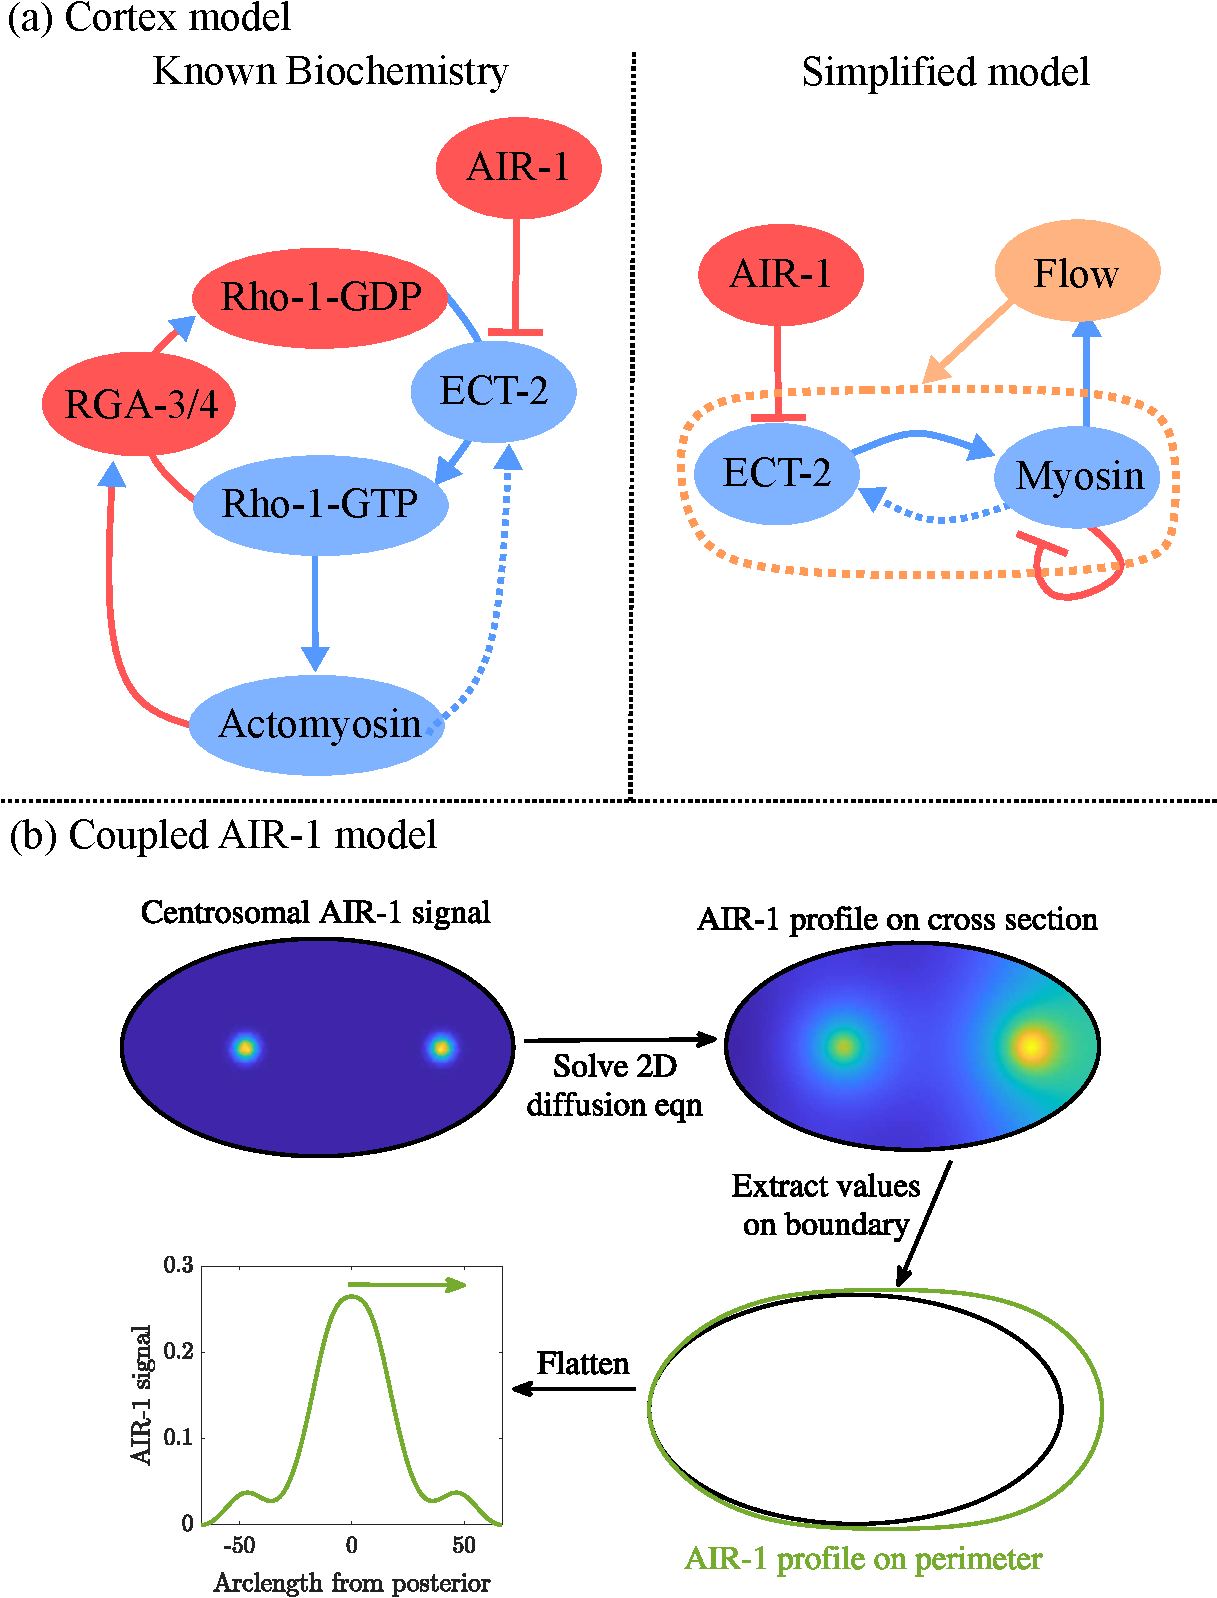
\includegraphics[width=0.9\textwidth]{BasicModel.pdf}
\caption{\label{fig:ModelSch}Modeling schematic for this study. (a) The model of the cortex, with the known biochemistry on the left and our simplified model on the right. This model takes the AIR-1 signal as input, and the equations are given in \eqref{eq:MyDim}. (b) Procedure for determining the AIR-1 signal. Given centrosome positions (shown are centrosomes in cytokinesis in wild-type embryos), we solve for the AIR-1 profile on the cross section using equation\ \eqref{eq:CD}, then formulate a one-dimensional AIR-1 profile by extracting the values on the boundary.}
\end{figure}

The general schematic of our model (as well as how it corresponds to the known biochemistry) is shown in Fig.\ \ref{fig:ModelSch}(a), and the mathematical details are presented in Appendix \ref{sec:MyModel}. AIR-1 inhibits ECT-2, and ECT-2 activates myosin (through Rho). Myosin feeds back on ECT-2 through direct recruitment, and through advection by flows. Finally, there is delayed negative feedback of myosin accumulation (through RGA-3/4-dependent inactivation of RHO-1) \citep{michaux2018excitable}. To constrain unknown model parameters, we incorporate known experimental measurements for the turnover rates of each molecule and flow speeds, and further assume that 
\begin{enumerate}[noitemsep, nolistsep]
\item 10\% of ECT-2 is bound to the cortex at steady state in wild-type embryos (our own unpublished(?) measurements). 
\item 30\% of myosin is bound to the cortex at steady state in wild-type embryos \citep[Fig.~S3j]{gross2019guiding}.
\item There is a modest increase (two-fold) in the recruitment rate of ECT-2 due to cortial myosin, in a myosin concentration-dependent manner.
\end{enumerate}
In the Appendix, we use these assumptions to constrain all of the model parameters. Our specific procedure is to impose a certain ECT-2 or myosin profile, and adjust the parameters until we get the desired steady state of the other species. \red{REVISE: In doing so, we show that ECT-2, due to its short residence time, can only take on the experimentally-measured profile if it is recruited by myosin, as opposed to being only advected. Talk about the excitability of the system and where our parameters sit.}

\subsection{Coupled model of AIR-1}
As an input to the cortex model, we solve for the AIR-1 profile on the boundary of a two-dimensional cross section of the embryo. Figure\ \ref{fig:ModelSch}(b) provides an overview of this process: for each embryo type, we obtain the centrosome positions, then solve a diffusion equation to obtain the AIR-1 profile on the entire embryo cross section. Evaluating the AIR-1 concentration (which has arbitrary units) on the boundary then gives a profile on the embryo perimeter, which we flatten out to a single periodic dimension. The mathematical details of this process are discussed in Appendix \ref{sec:AIR1D}; here it suffices to list the following assumptions that go into our model:
\begin{enumerate}[noitemsep, nolistsep]
\item During cytokinesis, the centrosomes have radius about 2 $\mu$m. The radius during polarization is 10\% of this.
\item AIR-1 is activated on the centrosomes.
\item Active AIR-1 diffuses towards the cortex according to Fick's law.
\item A global phosphatase activity inactivates AIR-1 throughout the cytoplasm. 
\end{enumerate}
Setting the level of global phosphatase activity is a non-trivial undertaking. As shown in Appendix \ref{sec:AIR1D}, low levels of phosphatase activity give high global AIR-1 levels, which translate to low ECT-2 levels everywhere. Such levels were shown to block psuedocleavage in centralspindlin-independent cytokinesis, due to low contractility \citep{afshar2010regulation, kotak2016aurora}. Our choice is to set the phosphatase activity so that centrosomes close to the posterior pole (in polarization) have a negligible AIR-1 concentration in the anterior ($< 1\%$ of the anterior concentration).

\section{Results}
In the absence of PAR proteins, it is known that the AIR-1/ECT-2 signal from the centrosomes leads to transient clearing of myosin from the posterior pole, and that the myosin profile reverts back to a uniform state after the centrosomes move towards the cell equator \citep[Fig.~2E]{gross2019guiding}. 

\subsection{The centrosome distance determines the strength of polarization \label{sec:airpol}}
In cell polarization, \emph{both} centrosomes sit very close to the posterior cortex (about 1 $\mu$m away \citep{cowan2004centrosomes}). The centrosomes have a smaller size (about 0.2 $\mu$m). They also contain substantially less total AIR-1; here we assume that the amount scales with the area, so that the amount of AIR-1 on each centrosome during polarization is 1\% of that for cytokinesis. 

\begin{figure}
\centering
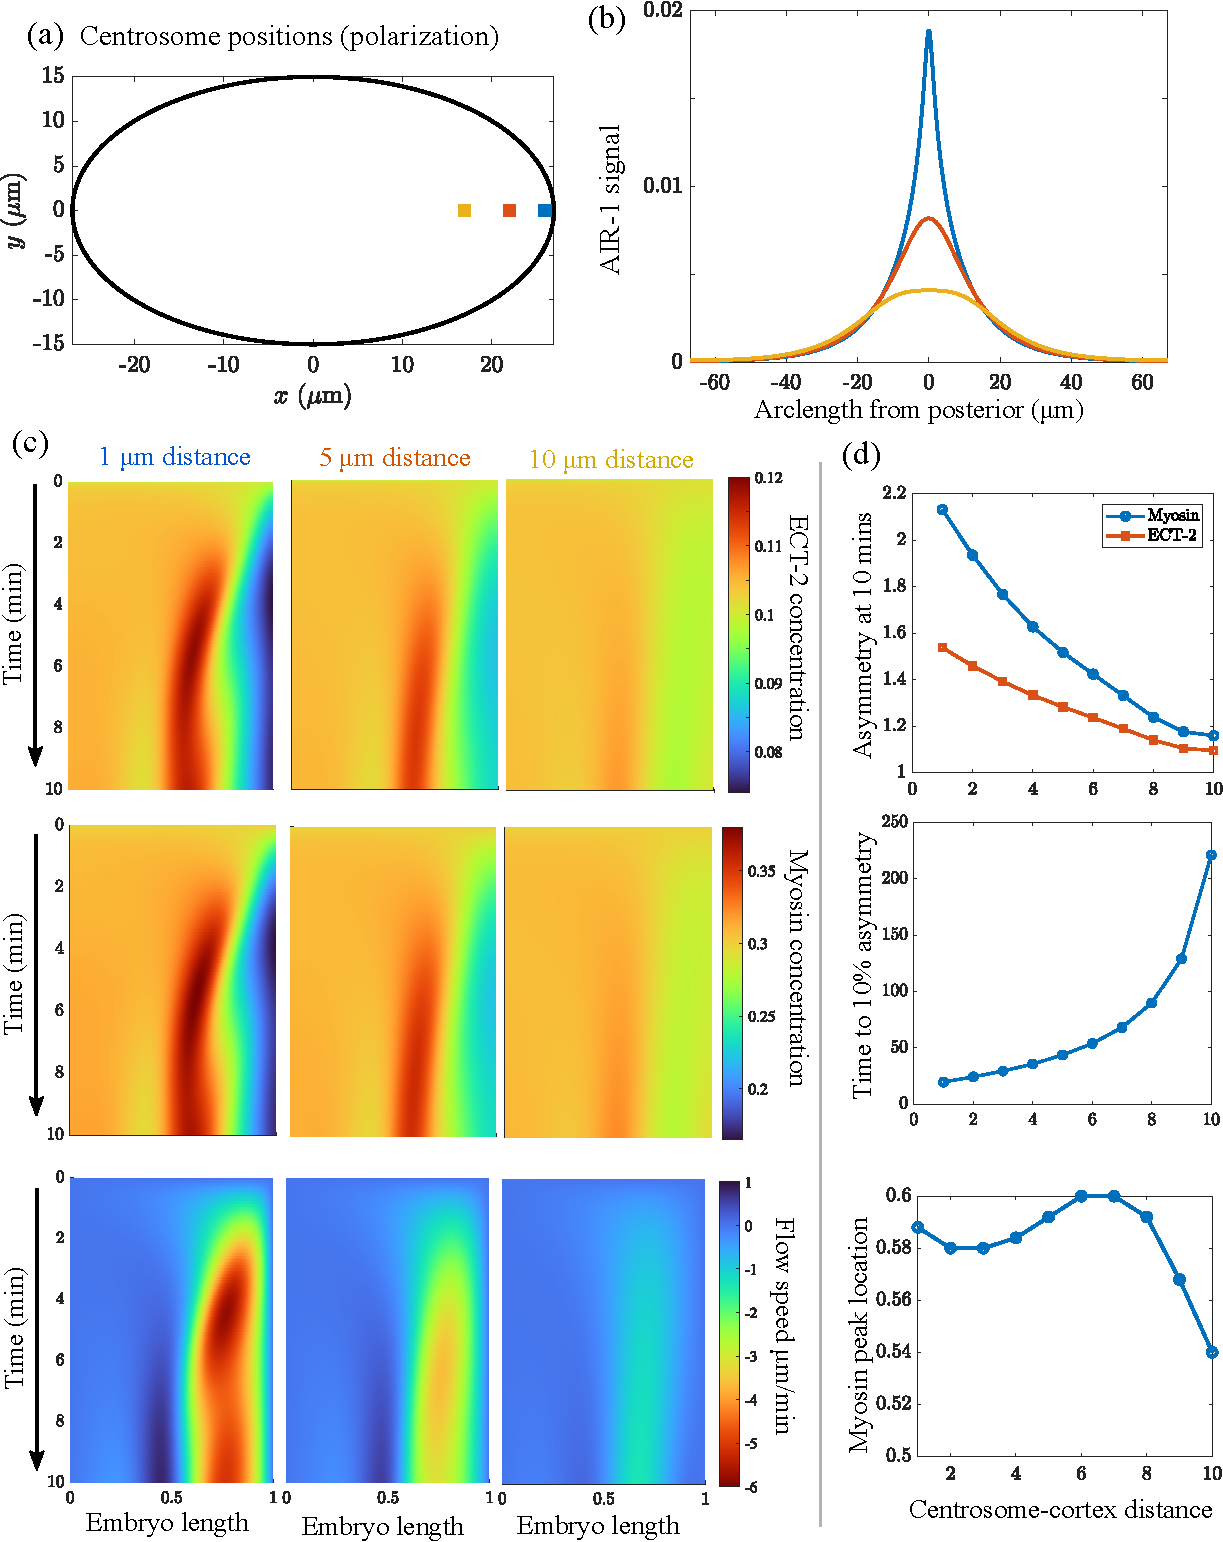
\includegraphics[width=0.9\textwidth]{PolarizationDists.pdf}
\caption{\label{fig:PolLoc}Centrosome locations set polarization dynamics. (a) The location of the centrosomes in our polarization simulations; we position both centrosomes 1, 5, and 10 $\mu$m away from the cell boundary. (b) The resulting AIR-1 signals along the cell perimeter. (c) The dynamics of polarization, starting from the uniform state, with the computed AIR-1 signal. We show the ECT-2 concentration (top), myosin concentration (middle), and flow speed (bottom) in a pseudo-kymograph, with time on the $y$ axis, and the A/P axis on the $x$ axis (A at left and P at right). \red{The 10\% asymmetry is for myosin.}}
\end{figure}

To explore the effect of centrosome distance and location, we position centrosomes at a distance 1, 5, and 10 $\mu$m from the posterior pole, and measure the resulting AIR-1 signal. There is a significant decrease in the AIR-1 signal as we move the centrosomes back from the cell boundary, with centrosomes 5 $\mu$m away giving a decrease of 50\% in AIR-1, and 10 $\mu$m giving an almost nonexistent AIR-1 signal.

Given these AIR-1 signals, we run the model forward in time to reach a steady state for polarization. Figure\ \ref{fig:PolLoc}(c) shows the trajectories of ECT-2, myosin, and the flow speed over ten minutes for the different centrosome positions. Under wild-type conditions, we predict an ECT-2 clearance (defined as the size of the region near the cue where $E < 0.095$) of about 20\% perimeter, which translates to roughly 10 $\mu$m on either side of the pole, in good agreement with experimental observations in PAR mutants \citep[Fig.~2E]{gross2019guiding}.\footnote{The model ``predicts'' an A/P asymmetry of at most 1.5 during polarization, which matches what we observed in previously \citep[Fig.~1]{longhini2022aurora}, but is calibrated to do so by changing the strength with which AIR-1 inhibits ECT-2.} The flow speed of at most 5--6 $\mu$m/min also matches observations in PAR mutants \citep[Fig.~2G]{gross2019guiding}. The time for peak clearance and asymmetries is delayed by a few minutes when the centrosomes move from 1 to 5 $\mu$m from the cortex \citep[Fig.~3F]{bienkowska2012centrosomes}, and centrosomes 10 $\mu$m away give no clearance at all. We also tested the case where centrosomes are positioned at the cell midline instead of the pole; these simulations yielded smaller ECT-2 asymmetries because of embryo geometry facilitating more diffusion of AIR-1. The difference was at most 10\%, however. 

\subsection{Effect of RGA Depletion}
\begin{figure}
\centering
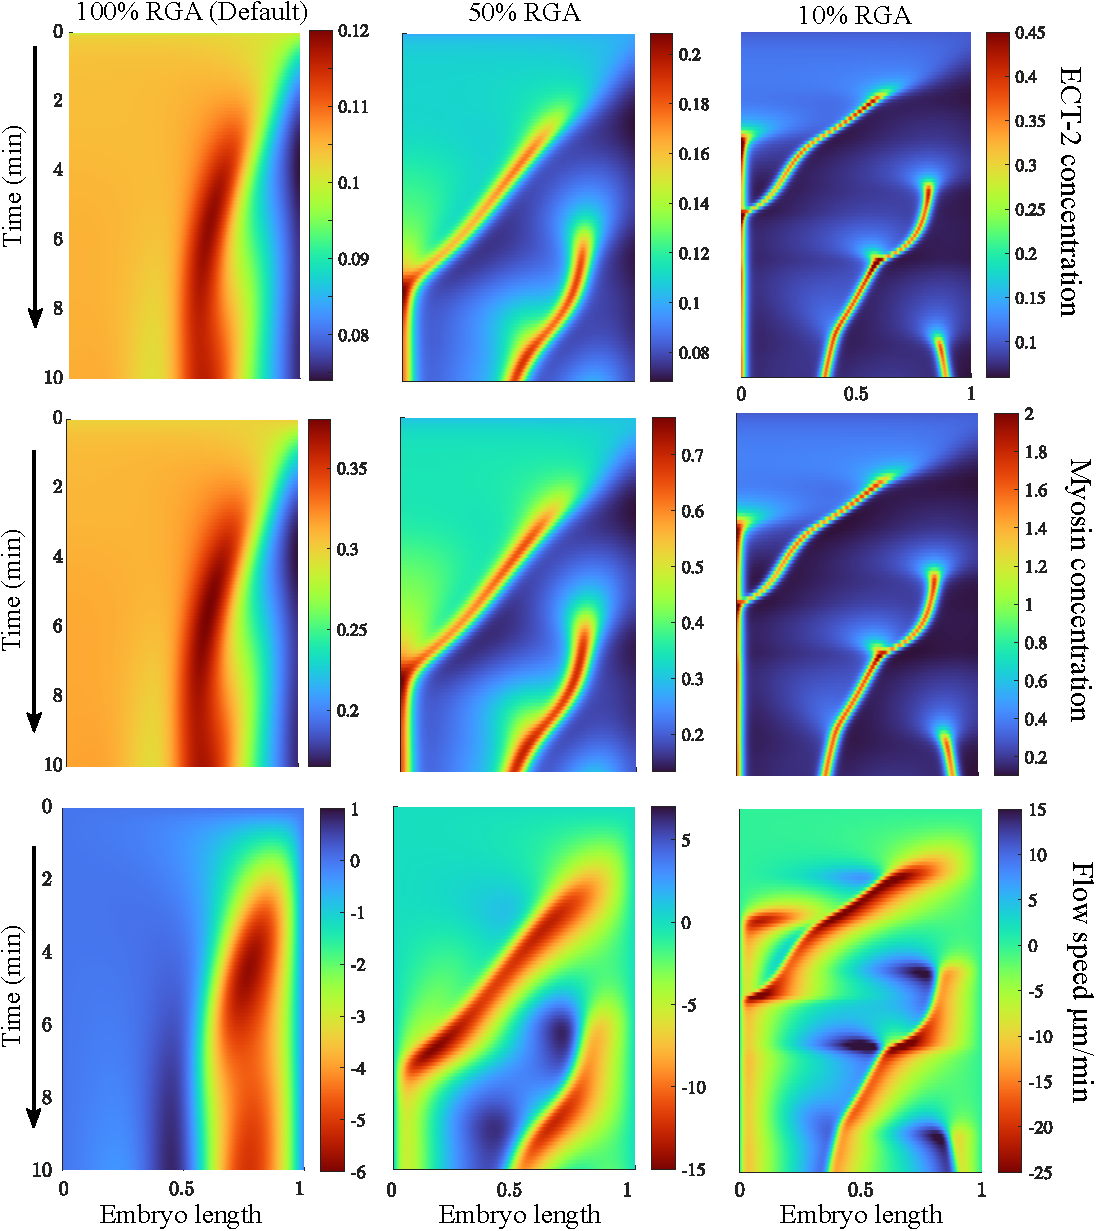
\includegraphics[width=\textwidth]{RGADepletion.pdf}
\caption{\label{fig:RGADepl}Dynamics when RGA is depleted. System is pushed into the excitable regime. The pulses contract faster, and form sooner, when there is less RGA.}
\end{figure}


\subsection{The relevance of rapid exchange}
We have shown that long-range reorganization of ECT-2 is possible despite its short residence time. The driver of this reorganization is recruitment by myosin, which is longer-lived on the cortex than ECT-2. Yet, is there any benefit to having rapid turnover of ECT-2 on the cortex? To explore this question, in Fig.\ \ref{fig:CueVsIC} we consider an alternative model where ECT-2 is advected, rather than recruited, by myosin. We accomplish this by making the ECT-2 lifetime an order of magnitude larger, and removing the recruitment by myosin from the model. In this case, we observe dynamics that are more chaotic. Initially (at $t=4$ mins), the ECT-2 and myosin distributions take on an asymmetry that matches that observed under normal conditions (Fig.\ \ref{fig:PolLoc}). After 5 minutes, however, the peak of myosin at 30\% length generates a strong flow which pulls ECT-2 from the posterior towards the anterior. This generates another minimum and a peak further towards the anterior, and we lose any notion of polarity. Thus when ECT-2 is advected, it can be pulled into the peak from both sides, resulting in additional myosin and additional flows which increase the size of the peak. By contrast, if ECT-2 is not advected, flows alone cannot concentrate ECT-2 into peaks, and the flow coming from the anterior is driven primarily by a local equilibrium where ECT-2 is depleted because of the AIR-1 signal. 

\subsection{A transient AIR-1 cue vs.\ local depletion}
\begin{figure}
\centering
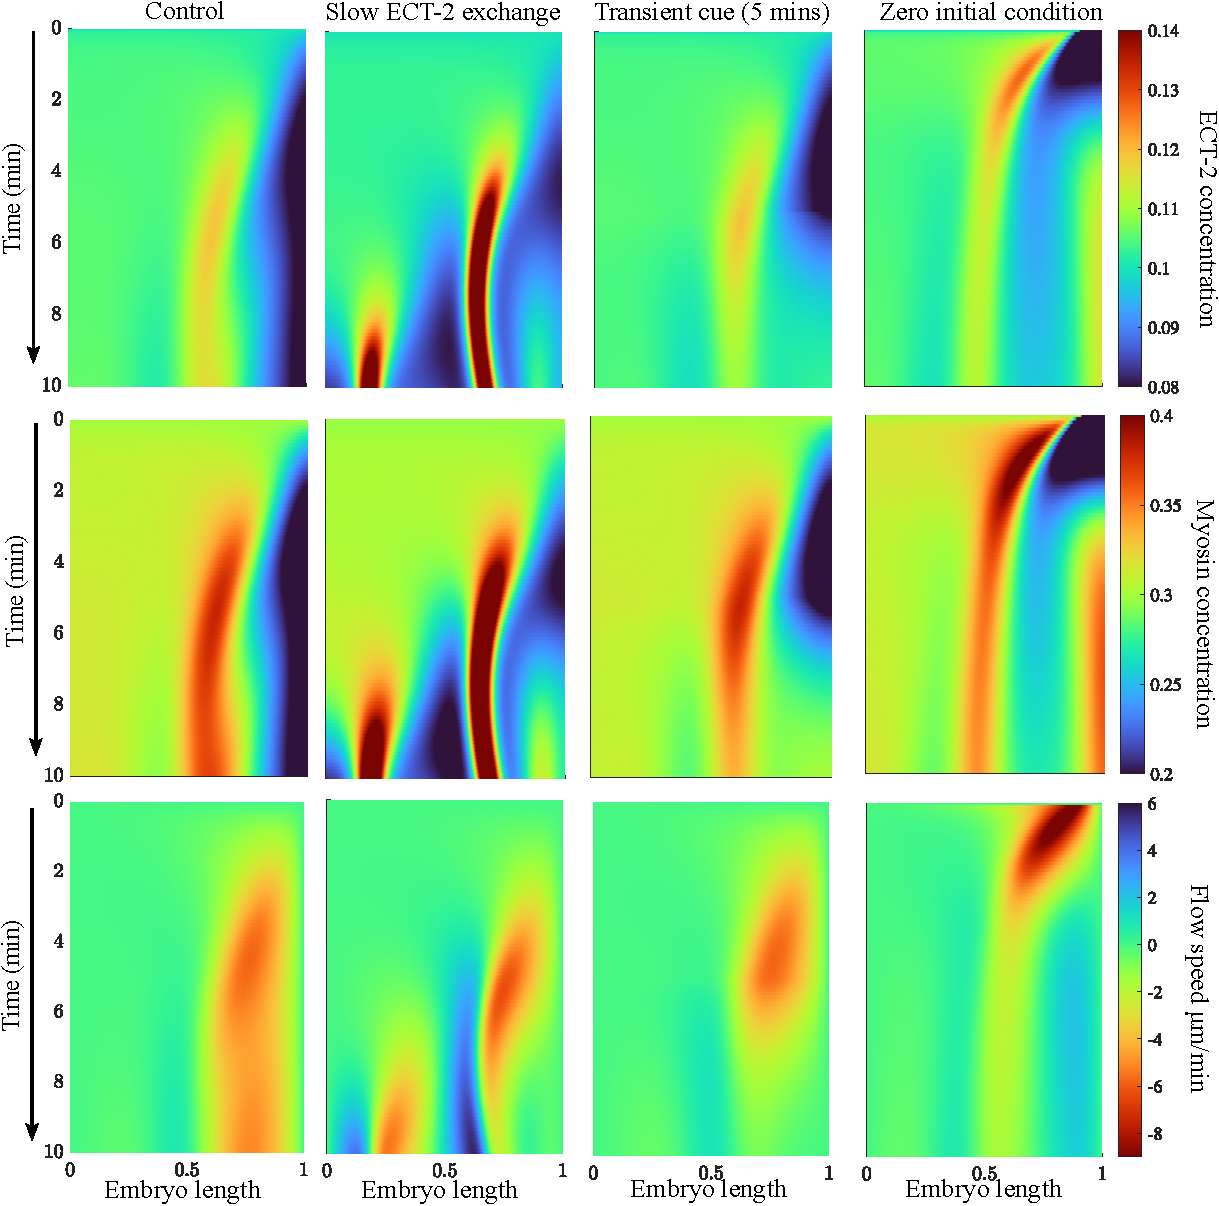
\includegraphics[width=0.8\textwidth]{PolarizationAdjust.pdf}
\caption{\label{fig:CueVsIC}Adjusting conditions in polarization. Left panel: adjusting parameters so that, rather than be recruited by myosin, ECT-2 has a ten-fold longer residence time and is only advected. (b) Simulating the case where the AIR-1 cue (blue in Fig.\ \ref{fig:PolLoc}) is applied for five minutes, after which we remove the AIR-1 signal and watch relaxation. (c) Simulating the case of no AIR-1 signal, but an initial condition that has 10\% of the domain at zero ECT-2 and myosin concentration. \red{Still need to fix this figure.}}
\end{figure}

What is the difference between a transient AIR-1 cue and an initial local depletion of ECT-2 and myosin at the posterior pole? To answer this question, we perform two simulations: one with the AIR-1 cue (centrosomes 1 $\mu$m from the posterior pole) active for five minutes, and a second with no AIR-1 cue and an initial unloading of myosin and ECT-2 at the posterior pole. The resulting dynamics over ten minutes are shown in Fig.\ \ref{fig:CueVsIC}. For the transient AIR-1 cue, the flow starts at zero, and steadily increases over five minutes time to give a flow speed of 6 $\mu$m/min. Turning off the cue then brings the flow speeds below 2 $\mu$m/min in three minutes time. By contrast, unloading myosin and ECT-2 from the posterior at $t=0$ triggers a similar set of flows towards the anterior, but the flows are maximal at $t=1$ minute, and then steadily decrease over time. Experimental data in PAR mutants show flows which are at a maximum almost immediately after polarity triggering, but the magnitude (5 $\mu$m/min) of these flows persist throughout polarity establishment phase (3--4 mins) \citep[Fig.~2G]{gross2019guiding}. Thus, the true situation is likely a combination of local unloading and a persistent AIR-1 cue. 


\subsection{Dynamics of cytokinesis}
In previous work \citep{longhini2022aurora}, we collected a series of data on how the ECT-2 accumulation on the posterior/anterior cortex during cytokinesis depends on the position of the corresponding centrosomes. In \citep[Fig.~7A]{longhini2022aurora}, these are presented as individual embryos; here we average the individual embryos for each of the nine treatments and show the mean values (error bars are a single standard error in the mean) in Fig.\ \ref{fig:CytoSit}(c, right panel). We highlight two important aspects of this ``S-shaped'' curve: on both the anterior and posterior cortex, there is a plateau in the ECT-2 accumulation. That is, it appears that above or below a certain distance, the ECT-2 accumulation does not depend at all on the centrosome proximity. By contrast, for distances in the range 10--20 $\mu$m, there is an ultra-sensitive dependence of the ECT-2 concentration on the proximity. 

\begin{figure}
\centering
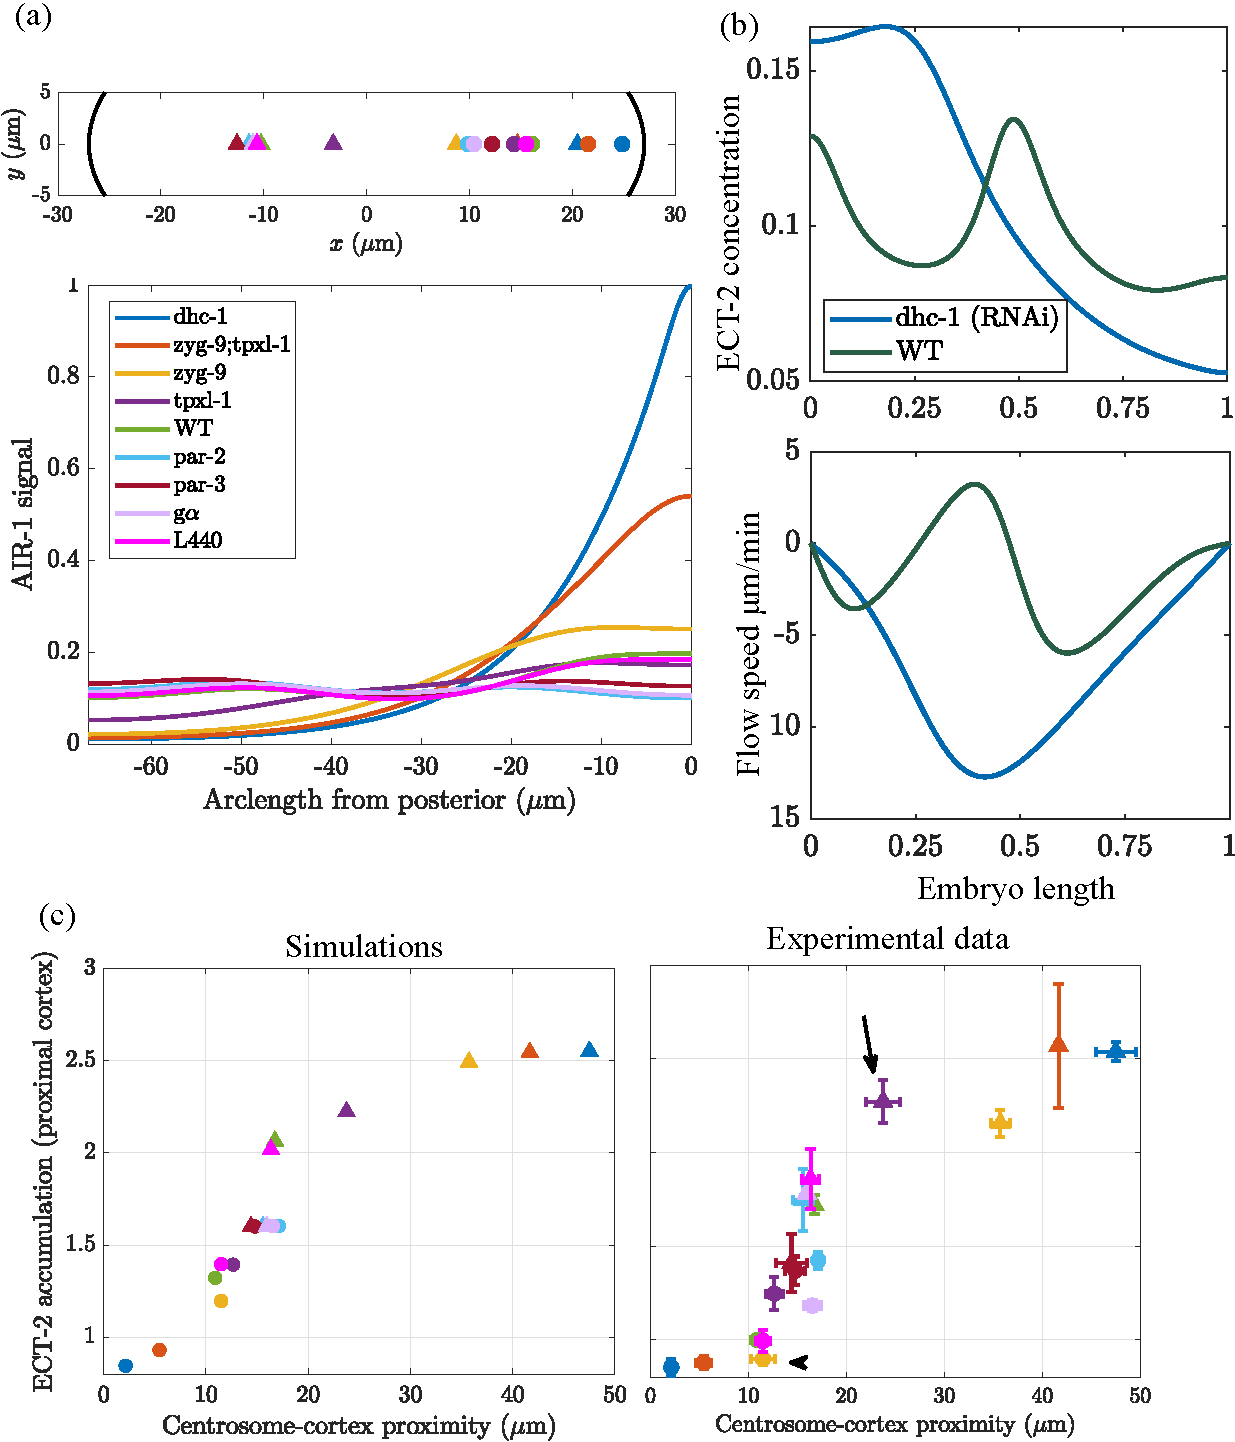
\includegraphics[width=\textwidth]{Cytokinesis.pdf}
\caption{\label{fig:CytoSit} Extending the model to cytokinesis. (a) The centrosome positions for each embryo treatment, which are inputs to the diffusion model, and the corresponding AIR-1 signal on the cell perimeter, obtained from solving the diffusion equation \eqref{eq:CD}. (b) Steady states (profiles after ten minutes)  in both dhc-1 (blue) and wild type (green) embryos. (c) The simulation results and experimental data for how the ECT-2 accumulation on the proximal cortex depends on the centrosome positions \citep[Fig.~7A]{longhini2022aurora}. }
\end{figure}

Using the centrosome positions measured in \citep{longhini2022aurora}, and repeated in Fig.\ \ref{fig:CytoSit}(a), we first compute the AIR-1 signal (in arbitrary units) along the cell perimeter for each of the embryo treatments. We notice the high posterior levels of AIR-1 in dhc-1 (RNAi) and zyg-9;tpxl-1 embryos, which stand out from the rest. Despite the differences in AIR-1 signal in the posterior, these two embryo types have the same posterior ECT-2 signal as zyg-9 embryos. In Appendix \ref{sec:MyIndModels}, we use this observation to inform a simple saturation model for the effect of AIR-1 on ECT-2. In particular, these observations suggest the effect of the AIR-1 signal saturates around $A_c=0.2$. 

We use the AIR-1 signals from Fig.\ \ref{fig:CytoSit} as inputs to the same cortex model (Fig.\ \ref{fig:ModelSch}(a)) that we parameterized under polarization conditions. Without changing any of the parameters, we simulate each embryo treatment to steady state, then record the ECT-2 concentration at the anterior/posterior pole at the time of the maximum asymmetry (approximately the steady state). Figure \ref{fig:CytoSit}(b) shows the steady state distribution of ECT-2 and the steady state flow speeds for dhc-1 (RNAi) and wild type embryos under cytokinesis conditions. The flows are of a realistic magnitude, and the ECT-2 concentration ratios between the anterior and posterior poles resemble the experimental measurements. Fig.\ \ref{fig:CytoSit}(c) shows the ECT-2 accumulation on the anterior/posterior pole across all embryo treatments. We observe a plateau at the low end, corresponding to saturation of the AIR-1 signal, and a plateau at the high end, where myosin accumulation and flow is inhibited by RGA 3/4. In the middle, we see an ultra-sensitive dependence: moving from 10--20 $\mu$m centrosome distance gives a roughly two-fold change in ECT-2 accumulation, similar to the experimental data in Fig.\ \ref{fig:CytoSit}(a). 

\subsection{Comparing cytokinesis vs.\ polarization}

\section{Discussion}

\begin{appendix}
\renewcommand{\thefigure}{S\arabic{figure}}
\renewcommand{\theequation}{S\arabic{equation}}
\setcounter{equation}{0}
\setcounter{figure}{0}

\section{Mathematical appendix} 

\subsection{AIR-1 diffusion model \label{sec:AIR1D}}
The contractility circuit is forced by a cue from the centrosomes which contain Aurora A (AIR-1), an inhibitor of ECT-2. We assume that the AIR-1 signal gets to the membrane by diffusion. Letting $a(\V x)$ be the concentration of AIR-1 in the two-dimensional embryo cross-section, we have the equation
\begin{subequations}
\label{eq:CD}
\begin{align}
\label{eq:DiffEqn}
\Delta a -\koffb a=  -f \qquad &\V{x} \in \Omega.\\
\label{eq:DiffBC}
\nabla a \cdot \V{n}=0 \qquad &\V{x} \in \partial \Omega,
\end{align} 
where\ \eqref{eq:DiffEqn} is the diffusion equation for the concentration and\ \eqref{eq:DiffBC} is a no-flux boundary condition through the boundary (here $\Omega$ represents the embryo area and $\partial \Omega$ represents the boundary). The signal $f(\V x)$ comes from the two centrosomes, which we model by Gaussian densities 
\begin{equation}
f(\V{x}) = \frac{C_0/D}{2 \pi \sigma_c^2}\sum_{i=1}^2\exp{\left(\frac{-\norm{\V{x}-\V{x}_i}^2}{2 \sigma_c^2}\right)}.
\end{equation}
Here $\V{x}_i$ is the location of the $i$th centrosome (typically at some location $(x_i,0)$), which changes depending on the embryo conditions. In addition to the centrosome location, the signal has two other parameters: $C_0/D$ is the strength of the cue (the integral of $f(\V{x})$ over the entire embryo cross-section, normalized by the cytoplasmic diffusion coefficient $D$), and $\sigma_c$ is the centrosome ``size'' (the standard deviation of the Gaussian, which is roughly half the size of the centrosome). For cytokinesis, the centrosomes have size about 2 $\mu$m, so we set $\sigma_c=1$ $\mu$m. In polarization, the centrosomes have size about 0.2 $\mu$m, so we set $\sigma_c=0.1$ $\mu$m. The signal strength $C_0/D$ is arbitrary; we set it to 1 for cytokinesis and 0.01 for polarization, thus assuming that the total amount of AIR-1 signal is proportional to centrosome area.
\end{subequations}
The diffusion equation\ \eqref{eq:DiffEqn} also contains a basal rate of inactivation of AIR-1 (phosphatase activity). This introduces another parameter which is the inactivation rate relative to the diffusion coefficient in the cytoplasm ($\koffb$, units $\mu$m$^{-2}$). 

We use a standard first-order finite element method to solve\ \eqref{eq:DiffEqn}. In brief, the elliptical domain of the embryo is meshed into nodes and triangles \citep{persson2004simple}, which define a set of linear Lagrangian basis functions $\psi_k$ that are 1 at node $\V{x}_k$ and 0 everywhere else. Multiplying\ \eqref{eq:DiffEqn} by a basis function $\psi_k$, then integrating by parts using the boundary condition\ \eqref{eq:DiffBC} gives 
\begin{equation}
\sum_j \int_{\Omega} \left(\nabla \psi_k \cdot \nabla \psi_j\right) a_j \, d\V{x}+\sum_j \int_{\Omega} \psi_k \psi_j a_j \, d\V{x}= \sum_j \int_{\Omega} \psi_k \psi_j f_j \, d\V{x},
\end{equation}
which can be written as the matrix equation $\left(\M K + \koffb \M M \right) \V a = \M M \V f$, where $\M{M}$ is the so-called mass matrix and $\M{K}$ the stiffness matrix for finite elements. These matrices are assembled using standard techniques \citep[c.~7]{gockenbach2006understanding}; see the github repository \url{https://github.com/omaxian/CElegansModel/} for code.

\subsubsection{Constraining level of AIR-1 phosphatase activity}
To constrain the level of phosphatase activity (parameter $\koffb$), we compute the profile of AIR-1 under polarization conditions (both centrosomes 1 $\mu$m from the posterior pole, with $C_0/D=0.01$), and plot the resulting AIR-1 signal in Fig.\ \ref{fig:AIR1ProfKoff}. When the phosphatase activity is low, the no flux boundary condition traps AIR-1 inside the embryo, and the relative difference between posterior and anterior is small. Increasing the phosphatase activity disproportionately lowers AIR-1 levels on the anterior pole (since it is much farther from the centrosomes). We assume that anterior levels of AIR-1 during polarization are at most 1\% of posterior levels; this constrains $\koffb=10^{-2}$. 

\begin{figure}
\centering
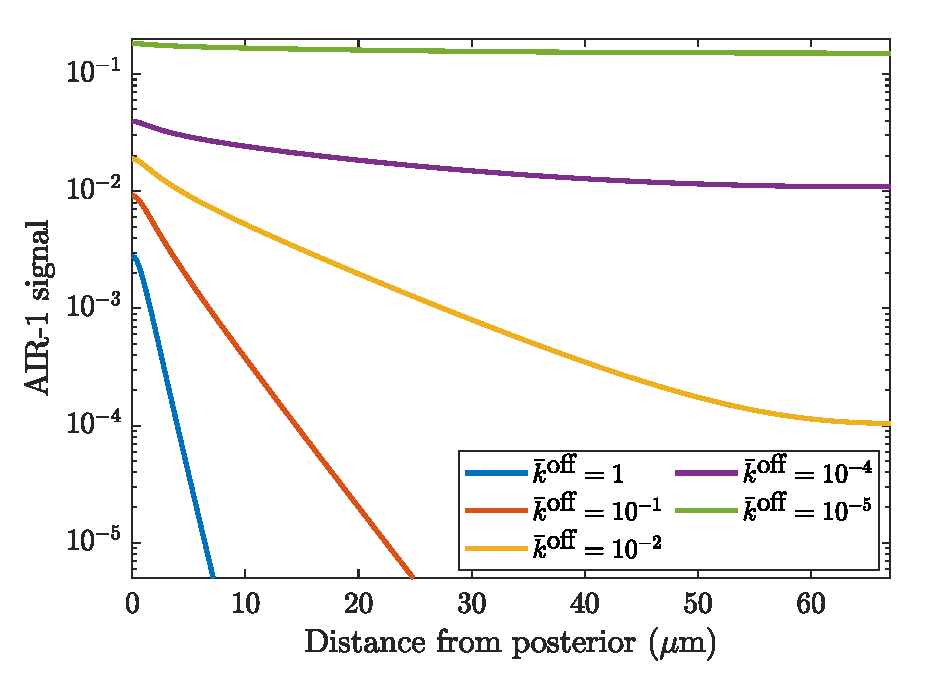
\includegraphics[width=0.6\textwidth]{PolarizationKoffAir.eps}
\caption{\label{fig:AIR1ProfKoff}AIR-1 signal vs.\ distance from posterior under polarization conditions (blue squares in Fig.\ \ref{fig:PolLoc}(a)). We vary the level of phosphatase activity $\koffb$ until the posterior level is less than 1\% of the anterior level, settling on $\koffb=10^{-2}$ $\mu$m$^{-2}$.}
\end{figure}


\subsection{ECT-2/Myosin circuit \label{sec:MyModel}}
We here formulate the equations for the model shown in Fig.\ \ref{fig:ModelSch}(a), where ECT-2 (through activating $\rho$) activates myosin at the cortex. To minimze the number of parameters, we consider a simplified version of the true dynamics (where ECT-2 signals myosin by activating rho) and formulate a model with two variables, $E$ (for ECT-2) and $M$ (for myosin). In dimensional units (denoted by hats), the equations we use are 
\begin{subequations}
\label{eq:MyDim}
\begin{gather}
\partial_{\hat t} \hat E + \partial_{\hat x} \left( \hat v \hat E\right) = \hat D_E \partial_{\hat x}^2 E +\kon_E \left(1+k_\text{ME} \hat M\right)\hat E_c - \koff_E  \left(1+k_\text{AE}\left( \frac{\hat A}{\hat A_c+\hat A}\right)\right)\hat E \\
\partial_{\hat t} \hat M +\partial_{\hat x} \left( \hat v \hat M\right)  = \hat D_M \partial_{\hat x}^2 M +k_\text{EM} \hat E ^2 \hat M_c - \koff_M \hat M -k_\text{fb} \hat M^4 \\
\label{eq:veleqn}
\gamma \hat v = \eta \partial_{\hat x}^2 \hat v +\hat \sigma_0 \partial_{\hat x} \hat M \\
\label{eq:CytoDim}
\hat E_c = \frac{1}{hL}\left(\Tot{E}L-\int_0^L \hat E(\hat x) \, d\hat x\right), \qquad \hat M_c =\frac{1}{hL}\left(\Tot{M}L-\int_0^L \hat M(\hat x) \, d \hat x\right).
\end{gather} 
\end{subequations}
Each of the species ECT-2 and myosin evolves by
\begin{enumerate}[noitemsep, nolistsep]
\item \emph{Advection by cortical flows.}  These are the terms $\Dx (v E)$ and $\Dx (v M)$.
\item \emph{Diffusion in the cortex.} These are the terms $D_E \Dx^2 E$, and $D_M \Dx^2 M$.
\item \emph{Binding to the cortex.} For ECT-2, there is a basal binding rate plus a linear enhancement by myosin. For myosin, the binding rate is proportional to the square of the ECT-2 concentration, without a basal binding rate. The motivation for this term is that myosin asymmetries are typically much stronger than ECT-2 asymmetries \citep{longhini2022aurora, munro2004cortical, mayer2010anisotropies}, and thus some nonlinearity is required. We choose the minimal such nonlinearity (see \citep[Eq.~(1)]{michaud2022versatile} for another choice, where Rho is represented explicitly). The binding rate is also proportional to the cytoplasmic concentration of each protein, defined in\ \eqref{eq:CytoDim}, where $L$ is the domain length, $h$ is the cytoplasmic ``thickness'' (so that $hL$ is the total area), and $\Tot{A}$ is the concentration of protein $A$ when all of it is bound to the cortex \citep{lang2022oligomerization}.
\item \emph{Unbinding from the cortex.} For ECT-2, the unbinding rate is composed of a basal rate expressing the fast exchange of ECT-2, plus inhibition by AIR-1 according to\ \eqref{eq:EctASat}. Myosin unbinds with a basal rate (expressing the combination of inactivation and unbinding), which is enhanced by delayed negative feedback (the $M^4$ term). The form of this term is a coarse-grained version of previously-published work \citep{michaux2018excitable}. The model there considered rho ($\rho$) and RhoGAP ($r$) as the unknowns, with the production of RhoGAP proportional to $\rho^3$ and the inhibition of $\rho$ proportional to $r \rho/(K+\rho)$. Here we coarse-grain this model into a single term, with the inhibition proportional to $M^4$. 
\end{enumerate}
Finally, the velocity equation \eqref{eq:veleqn} expresses the balance of active stress (which we assume is proportional to myosin concentration) with viscous stress and frictional resistance \citep{mayer2010anisotropies}. 

\subsubsection{Non dimensionalization}
Because absolute concentrations are unknown, it is easiest to assign values to unknown parameters when they are in dimensionless form. To do this, we non-dimensionalize so that length is in units of the embryo perimeter $L$, time is in units of the bound myosin lifetime $1/k^\text{off}_M$, velocity is in units of $\sigma_0/\left(\sqrt{\eta \gamma}\right)$ \citep{bois2011pattern} and concentration of species $A$ is in units of $\Tot{A}$. This gives new dimensionless variables 
\begin{subequations}
\label{eq:MySimple}
\begin{equation}
\label{eq:NDD}
x = \hat{x}/ L \qquad t=  \hat t \koff_M \qquad M= \hat{M}/\Tot{M}  \qquad E= \hat{E}/\Tot{E} \qquad v = \hat{v}/\left( \frac{\hat \sigma_0}{\sqrt{\eta \gamma}}\right),
\end{equation}
and a corresponding set of equations
\begin{gather}
\Dt E + \sigma_0 \Dx \left( v E\right) = D_E \Dx^2 E +\Kon_E \left(1+\Kme M\right)E_c - \Koff_E  \left(1+\Kae \left(\frac{A}{A_c+A}\right)\right)E \\
\label{eq:MyEq}
\Dt M + \sigma_0 \Dx \left( v M \right) = D_M \Dx^2 M +K_\text{EM} E ^2M_c - M -\Kfb M^4 \\
\label{eq:veleqn}
v = \ell^2 \Dx^2 v +\ell \Dx M \\
E_c = 1-\int_0^1 E(x) \, dx \qquad M_c = 1-\int_0^1 M(x) \, dx.
\end{gather} 
The conversion from dimensional to dimensionless form is straightforward for most of these parameters. Since some (e.g. $\Kae$, $\Kme$) are unknown anyway, it is not useful to report how they relate to the dimensional parameters. There are some important parameters to highlight, however. In flow patterns, $\ell=\left(\sqrt{\eta/\gamma}\right)/L$ is a hydrodynamic lengthsale (scaled by domain perimeter) expressing the connectivity of the cortex; local disturbances in myosin will typically propagate at most a distance $\ell$. The parameter $\sigma_0 = \hat \sigma_0/\left(L\koff_M \sqrt{\eta \gamma}\right)$ expresses the strength of the flows; the dimensional velocity in $\mu$m/s can be extracted by taking $v \times \sigma_0 L \koff_M$. 

\end{subequations}

\subsubsection{Numerical solution}
We use standard numerical methods to solve \eqref{eq:MySimple}. We discretize the one-dimensional domain at $N$ points with spacing $1/\Delta x$, and define the centered differentiation matrix $\M{D}$ and standard three points Laplacian differentiation matrix $\M{\Delta}$. Given the myosin profile at time step $n$, we first compute the velocity $v^{(n)}$ by solving $v^{(n)} = \ell^2 \M{\Delta} v^{(n)} + \ell \M{D} M^{(n)}$. Once the velocity is computed the ECT-2 and myosin equations are solved by combining a first-order upwind finite volume scheme for the advection terms \citep[Sec.~1.4]{hundsdorfer2003numerical} with implicit treatment of the diffusion terms (using the standard three point Laplaian). The reaction terms are all treated explicitly, and time-stepping is first order accurate. Matlab code  is available at the github repository \url{https://github.com/omaxian/CElegansModel/}.


\subsubsection{Parameter estimation}
Some of the parameters, as listed below, can be determined directly from experimental measurements, 
\begin{enumerate}[noitemsep, nolistsep]
\item The embryo cross section is an ellipse with approximate radii 27 $\mu$m and 15 $\mu$m, which gives a perimeter $L=134.6$ $\mu$m \citep{goehring2011polarization} .
\item The variable $\ell$ is the hydrodynamic lengthscale. In dimensional units, this was measured to be approximately 13 $\mu$m \citep{mayer2010anisotropies}, which means $\ell = 0.1$ in \eqref{eq:MySimple} (10\% domain perimeter).  
\item The myosin bound lifetime is about 15 s, so $\koff_M=1/15$ s$^{-1}$.
\item We assume that all species have a dimensional diffusion coefficient $\hat D_{E/M}=0.1$ $\mu$m$^2$/s \citep{goehring2011polarization, gross2019guiding, robin2014single}. Rescaling length by $L$ and time by $\koff_M$ gives a dimensionless coefficient $D_E=D_M=0.1/(L^2 \koff_M)=4.6 \times 10^{-5}$. 
\item The ECT-2 lifetime was measured using FRAP to be on the order of a few seconds \citep[Fig.~3D]{longhini2022aurora}. In cytokinesis, we set $\koff_E=0.33$/s, for a three second lifetime. Rescaling gives $\Koff_E=\koff_E/\koff_M=5$. The data show slightly faster recovery during polarization, so we increase $\koff_E$ by 20\% for those simulations.
%\item The value of $\Kme M$ determines what fraction of ECT-2 binding occurs from recruitment by myosin. We assume that 50\% of ECT-2 is recruited by myosin, so that $\Kme M = 1$. Because $M \approx 0.3$ (see assumption 7), we set $\Kme=1/0.3$. 
%\item The value of $\Kem E$ determined what fraction of myosin activation occurs via the ECT-2 pathway. We assume that 2/3 of myosin is activated by ECT-2, so that $\Kem E=2$. Because $E \approx 0.1$ (see assumption 7), we set $\Kem=20$. 
%\item In wild type embryos at steady state, we assume that 10\% of ECT-2 is bound to the cortex (our own unpublished(?) data), and 30\% of myosin is bound to the cortex \citep[Fig.~S3j]{gross2019guiding}.
\item For the negative feedback of myosin, we use the parameters determined in \citep{michaux2018excitable}. The feedback strength is obtained by assuming an equilibrium of RhoGAP in those equations (neglecting the basal binding rate which gives (in their notation) $$\Kfb=k_\text{GAP}\left(k_r^\text{ass}/k_r^\text{diss}\right)=0.1(0.245/0.047)=0.52\text{/s}$$. Rescaling by $\koff_M$ gives $\Kfb=7.8$ in our model. 
%\item According to our experimental data in Fig.\ \ref{fig:CytoSit}, the effect of the AIR-1 signal should saturate around $A \approx 0.2$. We therefore set $A_c=0.2$. 
\end{enumerate}
These assumptions give values for all parameters except for $\Kon_E$, $\Kme$, $\Kae$, $A_c$, $\Kem$, and $\sigma_0$. Four of these parameters can be fit by considering the desired model behavior in the absence of AIR-1. Experimental data \citep[Fig.~1]{longhini2022aurora} show that the A/P ECT-2 ratio is about 1.5:1, and that 10\% of ECT-2 is bound to the cortex. A similar set of data \citep[Figs.~S2,S3]{gross2019guiding} show that the A/P myosin ratio is about 2:1, with 30\% of myosin is bound to the cortex, and cortical flows on the order 10 $\mu$m/min. 

Figure\ \ref{fig:CortexMod} shows how we incorporate these data to fix the simulation parameters. First, as shown at left, we fix the ECT-2 profile according to experimental observations, then adjust $\Kem=50$ and $\sigma_0=0.2$, so that at steady state we obtain the myosin profile and flow speeds observed in experiments. Then, we recompute the steady state without inhibition by RGA, which results in a hypercontractile phenotype with more myosin in the anterior and larger flow speeds (dotted lines in bottom left plot), thus validating that our model gives qualitatively correct behavior. Similarly, in the right panel, we fix the myosin profile to correspond to experimental measurements, then adjust the parameters $\Kon_E$ and $\Kme$ until we obtain the correct ECT-2 profile (top right plots). In particular, in each case we set $\Kon_E$ so that 10\% of ECT-2 is bound to the cortex. Setting $\Kme=0$ (with $\Kon_E=0.66$) gives no recruitment of ECT-2 by myosin, and the ECT-2 profile is only shaped by advection, and is consequently barely asymmetric. Increasing to $\Kme=10/9$ (with $\Kon_E=0.5$) gives about 25\% of ECT-2 recruited by myosin and a larger asymmetry. We settle on $\Kme=10/3$ (with $\Kon_E=0.34$), which gives 50\% of ECT-2 recruited by myosin, and the 1.5:1 A/P ratio we seek. This completes the selection of all parameters, except for $\Kae$ and $A_c$. 

\begin{figure}
\centering
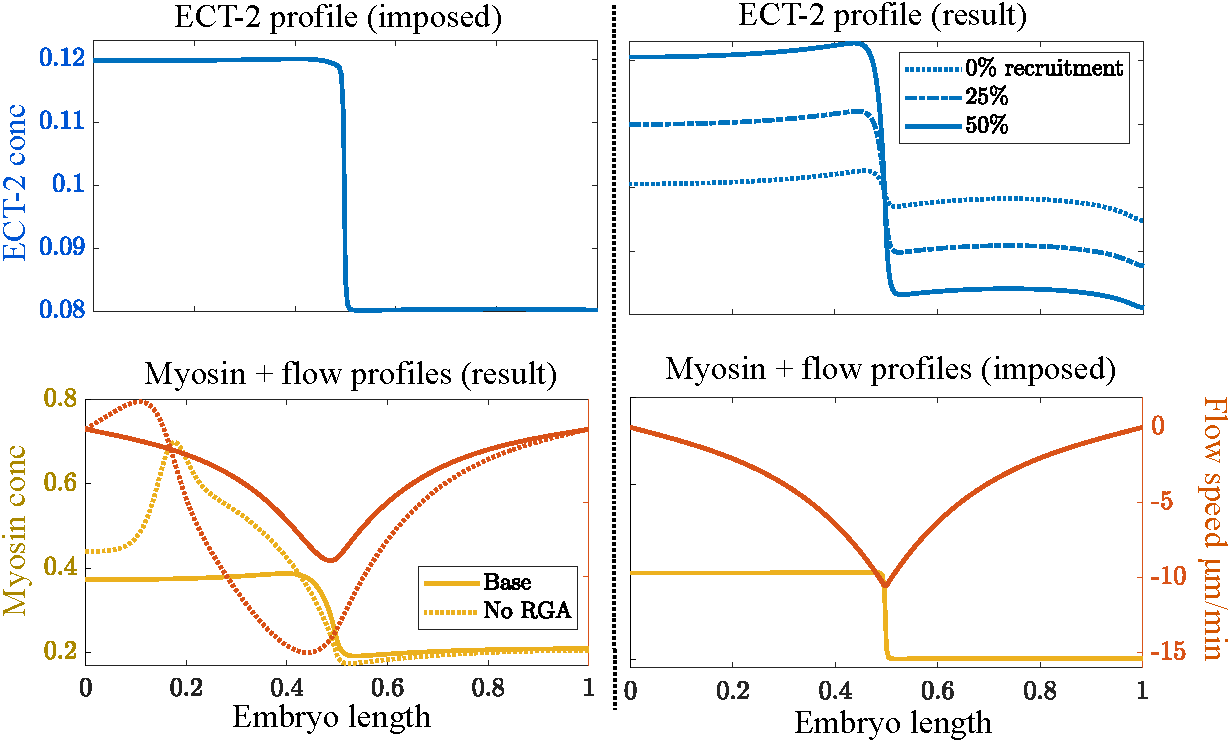
\includegraphics[width=\textwidth]{ModelValidation.pdf}
\caption{\label{fig:CortexMod}Validating our simple model of the cell cortex and setting the parameters. Left panels: we impose an ECT-2 profile that is 50\% higher on the posterior than anterior, then measure the myosin and flow profiles with our chosen parameters. Right: we impose the myosin and corresponding flow profile, and examine the ECT-2 profiles with different rates of myosin recruitment.}
\end{figure}

To select $\Kae=0.6$, we enforce that the max/min ECT-2 concentration is 1.5 under normal polarization conditions (left panel of Fig.\ \ref{fig:PolLoc}). The threshold $A_c$ does not come in during polarization because AIR-1 signals are low; as such we set its value according to the investigation in Section \ref{sec:MyIndModels}. 

\section{Supplemental investigations and figures}

\subsection{Linear stability analysis}
\begin{figure}
\centering
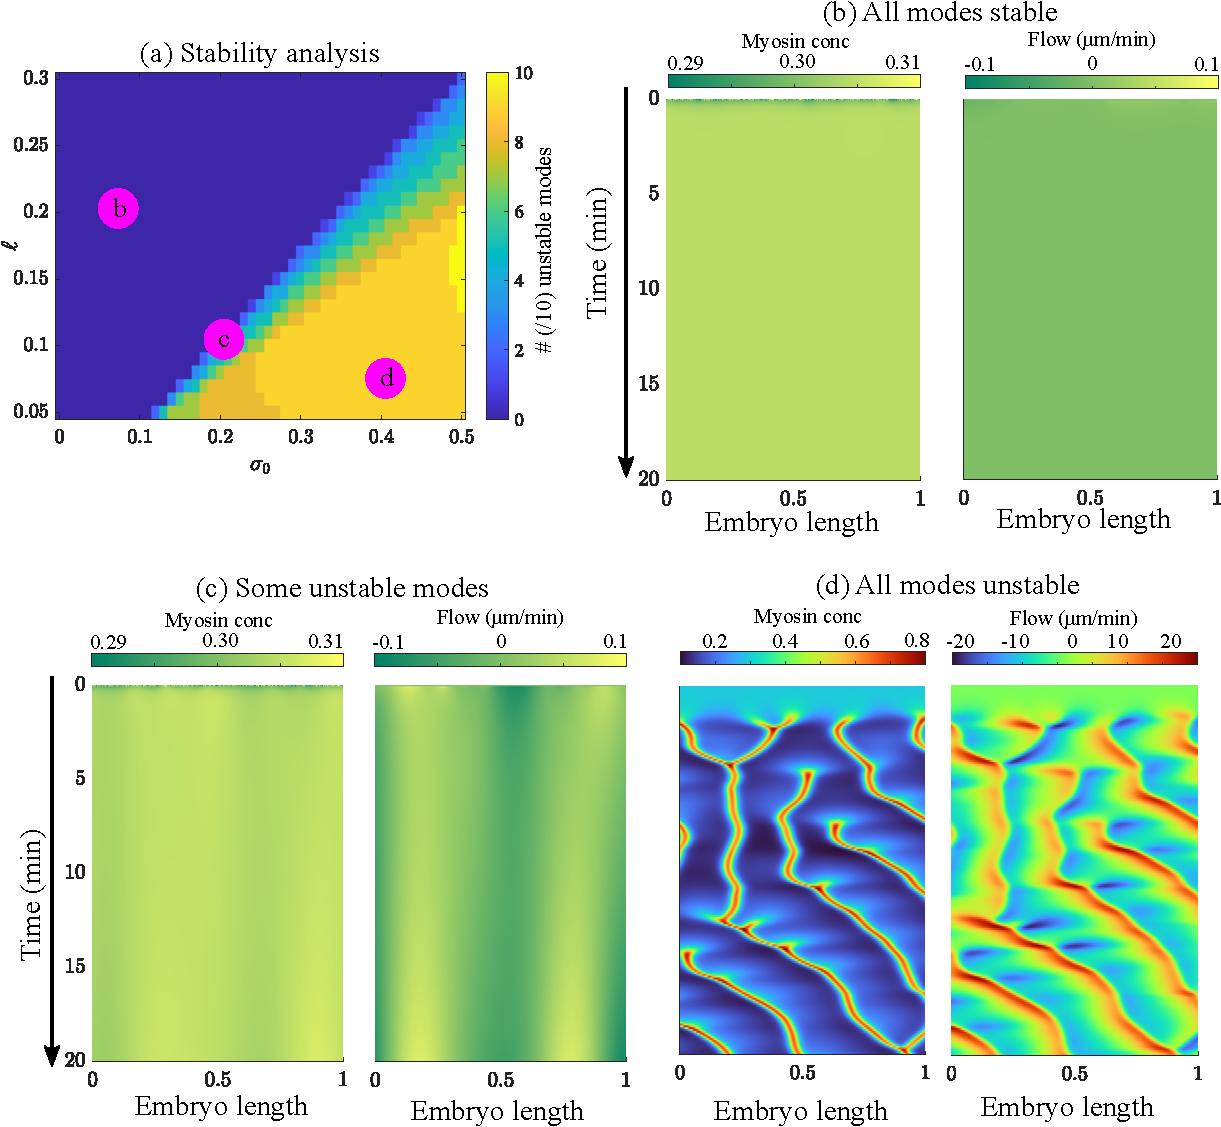
\includegraphics[width=\textwidth]{Stability.pdf}
\caption{\label{fig:Stability} Linear stability analysis of the uniform state. When all modes are unstable, pulses can form seemingly out of nowhere. This comes from a lengthscale long enough being depleted. The instability kicks in there. Pulses move apart, then new ones form.}
\end{figure}

\subsection{Parameter adjustments: polarization \label{sec:EctTurnP}}
In Fig.\ \ref{fig:CueVsIC}, we modify the parameters to examine an alternative hypothesis where ECT-2 has a longer lifetime. We consider in particular $\koff_E=1/25$ s$^{-1}$ (25 s residence time instead of 2.5) and $\Kon_E=0.068$ to give a 10\% bound ECT-2, and $K_\text{ME}=0$, so that myosin doesn't recruit ECT-2. All other parameters take their default values (in particular, $\sigma=0.2$). 

\subsection{Myosin-independent models for the ECT-2 response are inadequate \label{sec:MyIndModels}}
In the simplest possible model of ECT-2 dynamics, there is a local equilibrium of the binding rate and unbinding rate, where the latter increases in the presence of AIR-1,
\begin{equation}
\label{eq:EctA}
 \kon_E = \koff_E \left(1+\Kae A \right)E,
\end{equation}
and $\Kae$ expresses the strength of inhibition. This steady state model predicts that the ECT-2 concentration relates to the AIR-1 concentration at the cortex via
\begin{equation}
\label{eq:EctLinA}
E = \frac{\kon_E/ \koff_E}{ 1+\Kae A},
\end{equation}
which is a relationship with two unknown constants. Fitting these two unknown constants to the observed ECT-2 levels in dhc-1 (RNAi) embryos (where the AIR-1 signal is approximately 1 at the posterior and 0 at the anterior) gives $\kon_E/ \koff_E=2.55$ and $\Kae=2$. Substituting the AIR-1 levels from the other embryo treatments then gives the observed centrosome/ECT-2 accumulation plot shown in Fig.\ \ref{fig:LinFail}(a). There we see that the relationship \eqref{eq:EctLinA} correctly predicts saturation at low levels of AIR-1 (high centrosome-cortex distances), but fails to predict saturation at high AIR-1 levels (low distances) or ultra-sensitivity in between. 

\begin{figure}
\centering
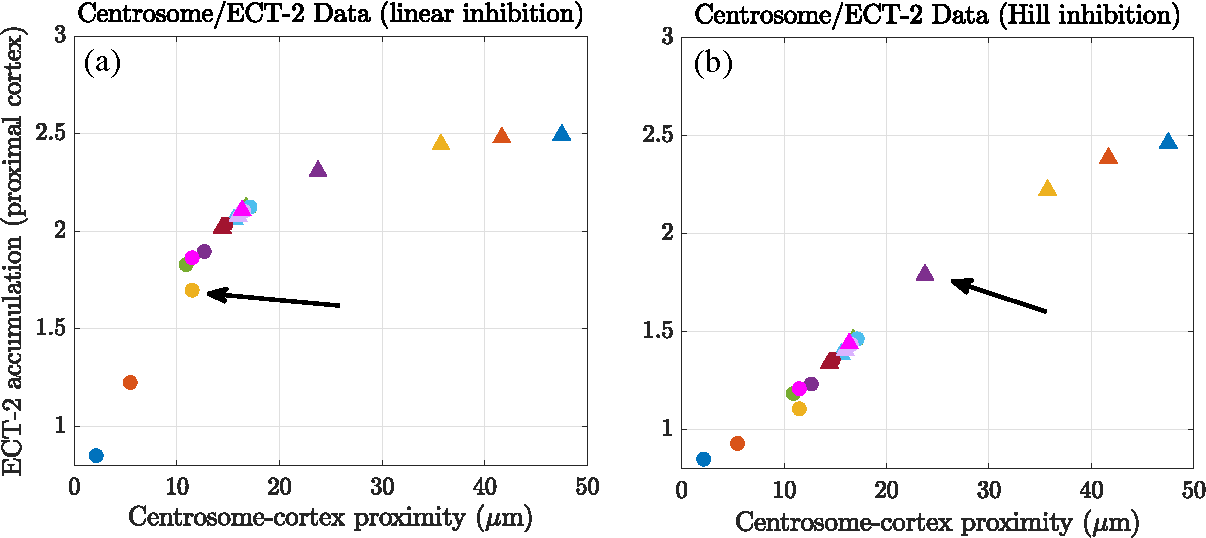
\includegraphics[width=\textwidth]{OtherAIRModelsCyto.pdf}
\caption{\label{fig:LinFail}Simple models based on AIR-1/ECT-2 inhibition fail to capture the experimental data on accumulation vs.\ centrosome position. We consider (a) a linear inhibition model \eqref{eq:EctLinA}, and (b) a linear model with saturation \eqref{eq:EctASat} (Hill function). Compared to the data in Fig.\ \ref{fig:CytoSit}, neither of these simple models capture the general S-shape of the curve, with plateaus at the low and high ends. }
\end{figure}

The AIR-1 signals we obtained in Fig.\ \ref{fig:CytoSit}(a) show that the AIR-1 signal at the posterior doubles when we switch from zyg-9;tpxl-1 (red) embryos to dhc-1 embryos (blue). Yet, the experimental data in Fig.\ \ref{fig:CytoSit}(a) show that the ECT-2 accumulation is unchanged. This tells us that there must be saturation in the AIR-1 inhibition dynamics; beyond some level, the amount of AIR-1 no longer impacts the inhibition strength. Based on the location of the plateau in the experimental data, it seems that this threshold level occurs around the posterior AIR-1 level in zyg-9 embryos, which our data in Fig.\ \ref{fig:CytoSit}(d) tells us is 0.2. Thus, we propose a new model where the local equilibrium is governed by 
\begin{equation}
\label{eq:EctASat}
 \kon_E = \koff_E \left(1+\Kae \left(\frac{A}{A_c+A}\right) \right)E,
\end{equation}
where $A_c=0.2$. Once again fitting $\kon_E/\koff_E=2.8$ and $\Kae=2.8$ to the data for dhc-1 embryos, we obtain the centrsome/ECT-2 plot shown in Fig.\ \ref{fig:LinFail}(b). There we see that we have correctly reduced the posterior ECT-2 levels in embryos with high AIR-1 signals to approach a plateau. However, we also reduce the ECT-2 levels in the other embryos (especially tpxl-1; purple), and we still no longer see the ulta-sensitivity in distances 10--20 $\mu$m. We propose that the failure of these simple models comes from a lack of propagation of the AIR-1/ECT-2 signal via flows. As shown in Fig.\ \ref{fig:CytoSit}(c), flows can exaggerate the smaller asymmetries, giving ultra sensitivity in the interior of the curve.


\end{appendix}

\bibliographystyle{plainnat}

\bibliography{../../PolarizationBib}


\end{document}
